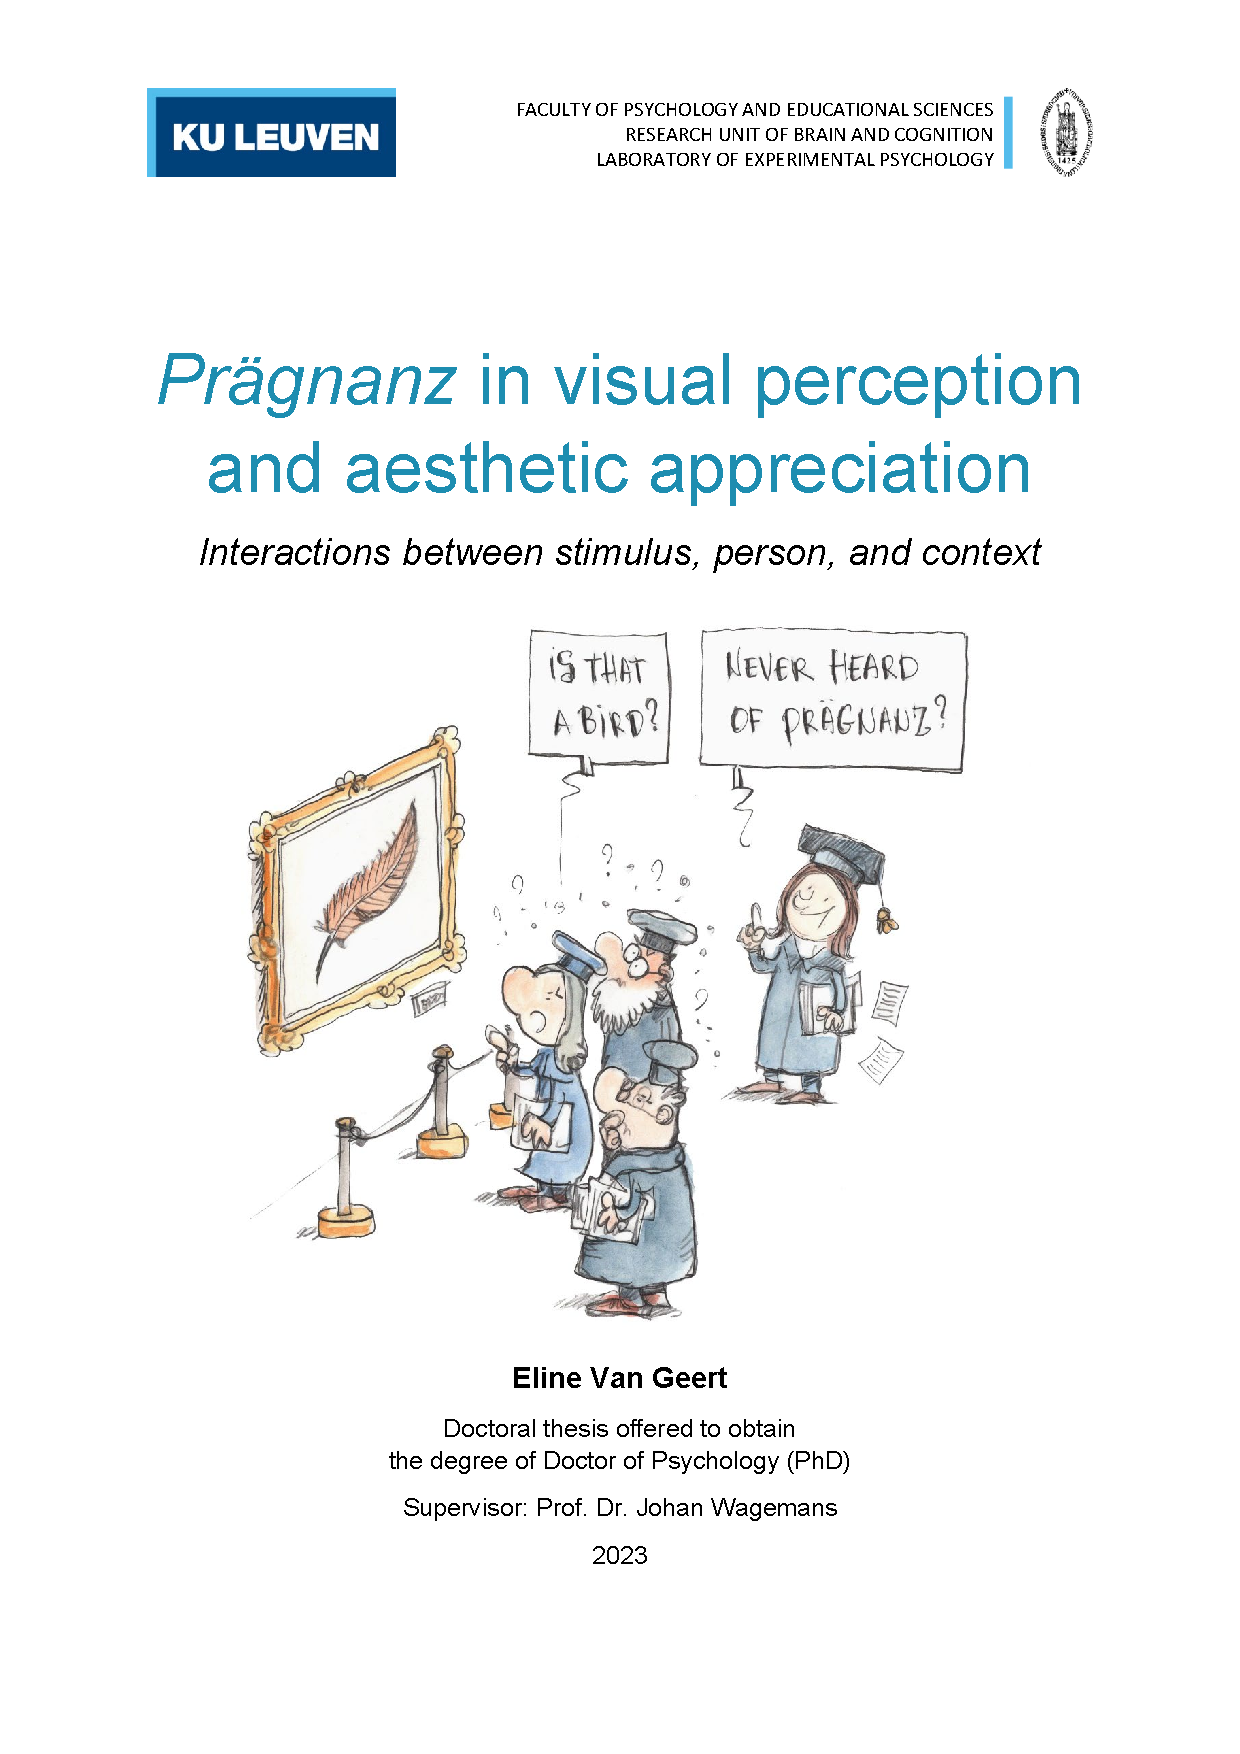
\includepdf[pages={1}, scale=1]{titlepage_thesis_EVG.pdf}
\clearpage\thispagestyle{empty}

\
\clearpage\thispagestyle{empty}
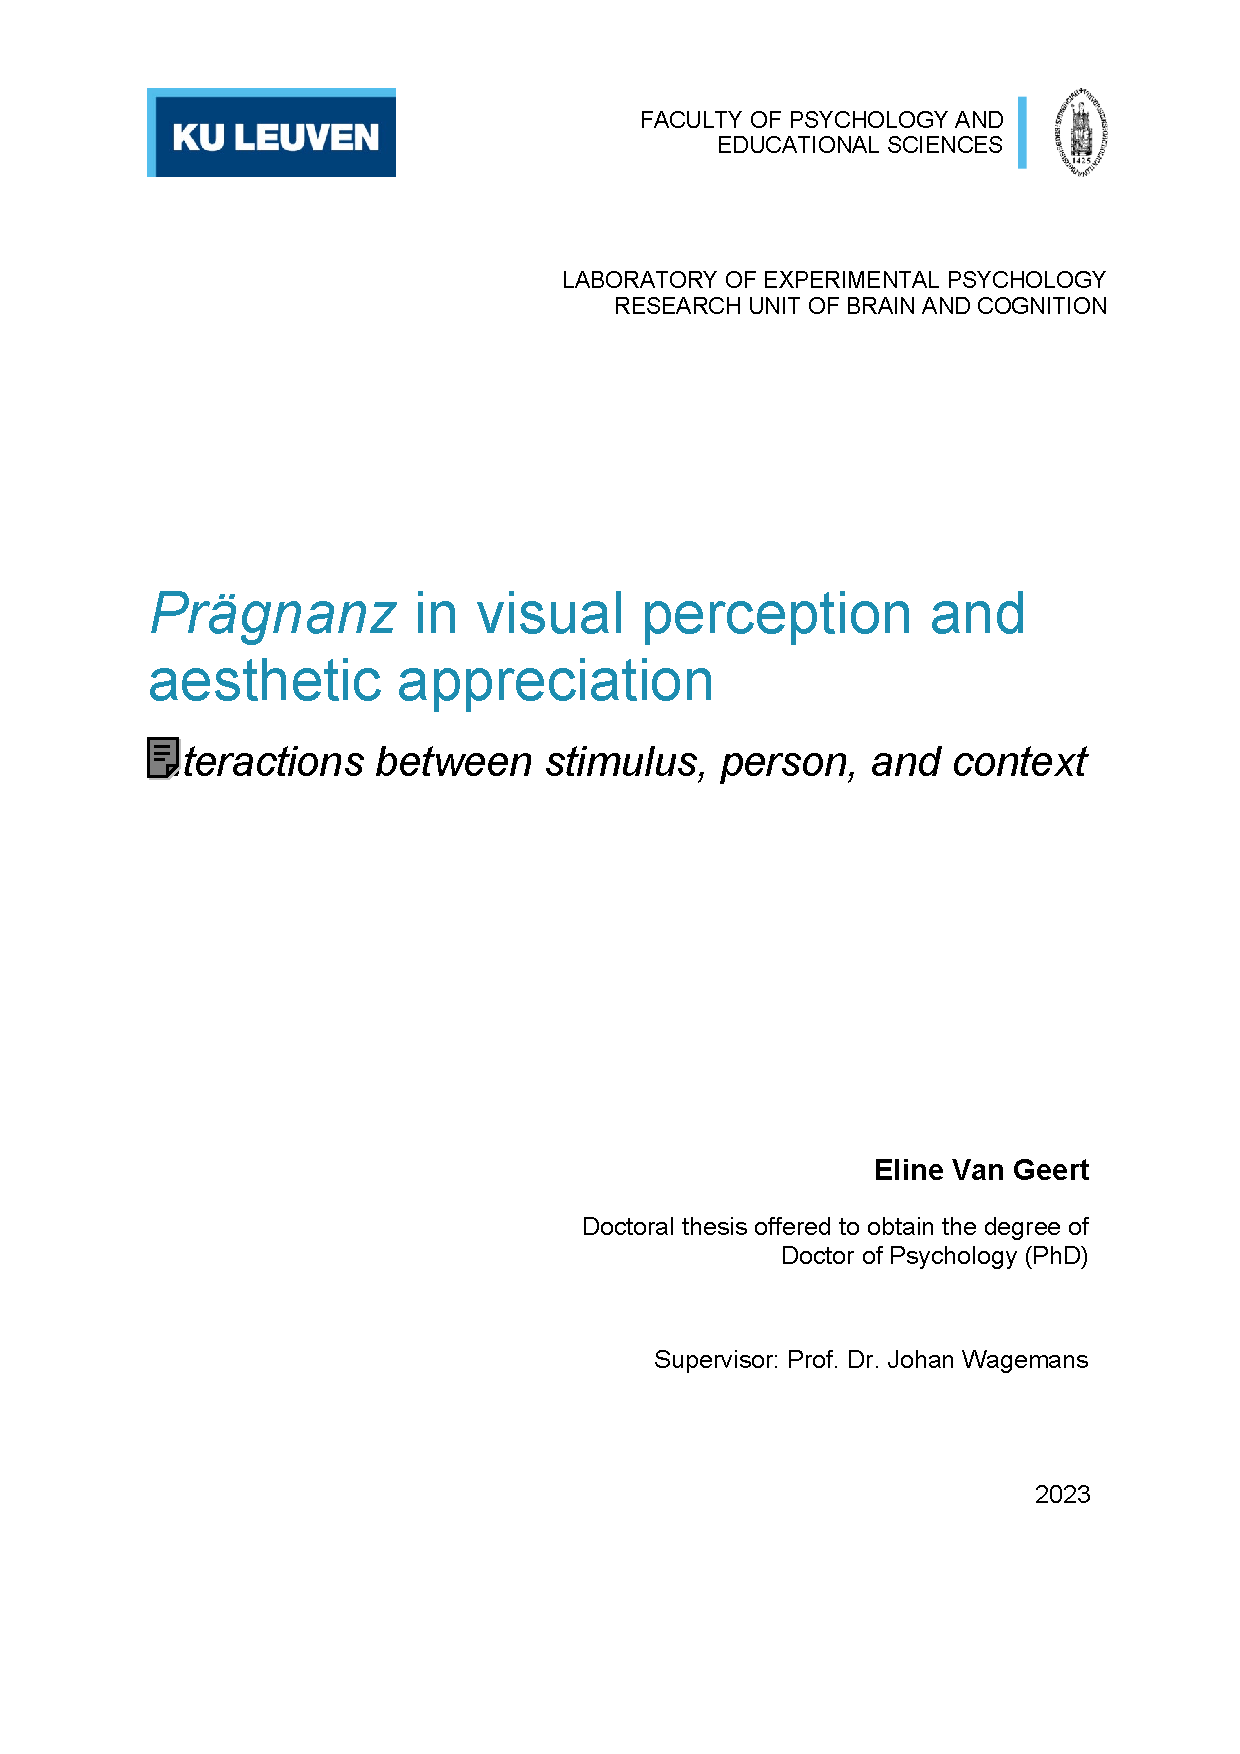
\includepdf[pages={1}, scale=1]{titlepage_thesis_EVG_firstpage.pdf}

\clearpage\thispagestyle{empty}

\vspace*{\fill}
\noindent
\copyright \ \ 2023, Eline Van Geert

\noindent
Cover illustration and illustrations at the start of each part were created by \href{http://jorissnaet.be/}{Joris Snaet}.

\noindent
This thesis was created using the \href{https://quarto.org/}{Quarto} publishing system. Both a \href{https://elinevg.github.io/pragnanz/doctoralthesis_EVG.pdf}{pdf version} and an \href{https://elinevg.github.io/pragnanz}{interactive HTML version} are available online \href{https://elinevg.github.io/pragnanz}{(https://elinevg.github.io/pragnanz)}. Online documentation appending some of the projects discussed in this dissertation can be found on the Open Science Framework \href{https://doi.org/10.17605/OSF.IO/7RSYF}{(https://doi.org/10.17605/osf.io/7rsyf)}. 

\setstretch{1.1}

\disableboldchapterintoc
\chapter*{Summary}
\addcontentsline{toc}{chapter}{Summary}

Things look as they do, not only because of the visual input an individual receives, but also because of the way in which the viewer organizes the input in a specific context (cf. Chapter~\ref{sec-introduction}). The law of \textit{Prägnanz} states that psycho-physical organization will always be as 'good' as possible given the prevailing circumstances. What does it mean for an organization to be 'good', however, and how do viewers clarify the incoming visual stimuli to achieve the best possible percept? 

A 'good' psycho-physical organization will contain at least some form of unity or regularity, and will become better when it is autonomous, complete, simple of structure, element rich, expressive, and/or meaningful (cf. Chapter~\ref{sec-pragnanzreview}). Prägnanz thus not only deals with purely figural aspects, but also with how purely and compellingly the phenomenal structure embodies an essence. Moreover, it comprises aspects related to both order and complexity. 

To achieve the best or clearest overall organization possible, human perceivers use \textit{internal representations of good Gestalts as reference points} to clarify the visual input. Whereas sometimes these reference points lead to increased \textit{sensitivity to change}, they can also act as robust magnets, decreasing perceptual distance between neighboring stimuli. In a first empirical study (cf. Chapter~\ref{sec-refpoints}), we show how the existence of strong internal reference points can explain differences in categorization, discrimination, and similarity judgments across a series of figures gradually transforming from one recognizable shape to another. 

If no strong pre-existing reference points are available that are similar enough to the incoming visual stimuli, the \textit{immediate context} can play a more extensive role in disambiguating the visual input. In a Registered Report using multistable dot lattices as stimuli (cf. Chapter~\ref{sec-rrdotlattices}), we confirmed differences in how individuals combine previous input and experience with current input in their perception, and showed stability of these individual differences over one to two weeks’ time. Furthermore, we developed an efficient Bayesian observer model that can predict both the \textit{attractive and repulsive} immediate context effects found in this task (cf. Chapter~\ref{sec-effbayesianmodel}).

\textit{How} will the internal reference points or the immediate context be used to clarify the incoming visual stimuli and arrive at a clearer, more prägnant percept? In every perceptual event, both simplification and complication will occur, albeit to a different extent depending on the strength of the internal and external conditions (related to the viewer and the visual input, resp.). Whereas unnecessary details, differentiating the visual input from the point of comparison, will be leveled or removed, important characteristics distinguishing the input from the reference will be emphasized. As we can conclude from our research, however, \textit{which} characteristics will be either superfluous or essential, and as a consequence which characteristics will be either \textit{simplified or complicated}, will partially depend on the context in which the stimulus is presented (cf. Chapter~\ref{sec-simplcompl}).

\textit{Order and complexity} are not only important aspects of Prägnanz, they also contribute to our experience of aesthetic appreciation. To improve reproducibility of research assessing the relation between order, complexity, and aesthetic appreciation in the visual modality, we developed the Order \& Complexity Toolbox for Aesthetics (OCTA; cf. Chapter~\ref{sec-octatoolbox}), a Python package and online application focused on creating multi-element displays varying on different order and complexity dimensions (e.g., shape, color, size of elements). Although primarily focused on aesthetics, OCTA can also be used in research on perceptual organization. Some first empirical studies using OCTA stimuli (not part of this dissertation) teach us that whereas order is almost never disfavored, the appreciation of complexity is more context-dependent. This relates closely to the core of Prägnanz: as some form of regularity is always required, how much intricacy a viewer can handle differs between contexts and individuals.

In sum (cf. Chapter~\ref{sec-conclusion}), to clarify and aesthetically evaluate visual stimuli, tendencies are at work that are both antagonistic and complementary: although they tend to decrease each other's influence, they also work together towards a better perceptual organization. What the optimal balance of both tendencies entails exactly will depend on the input the individual receives, the individual in question, the context in which the individual receives the input, as well as their interactions.

\clearpage\thispagestyle{empty}

\chapter*{Samenvatting}
\addcontentsline{toc}{chapter}{Samenvatting}

\setstretch{1.0}

Dingen zien er niet alleen uit zoals ze eruitzien vanwege de visuele input die een individu ontvangt, maar ook vanwege de manier waarop de kijker deze input in een specifieke context organiseert (cf. Hoofdstuk~\ref{sec-introduction}). De wet van \textit{Prägnanz} stelt dat psycho-fysische organisatie altijd zo 'goed' als mogelijk zal zijn gegeven de heersende omstandigheden. Wat betekent het echter voor een organisatie om 'goed' te zijn, en hoe verduidelijken kijkers de binnenkomende visuele prikkels om tot de best mogelijke waarneming ervan te komen?

Een 'goede' psycho-fysische organisatie zal op z’n minst een vorm van eenheid of regelmaat bevatten, en wordt beter wanneer ze daarnaast ook autonoom, volledig, eenvoudig van structuur, rijk aan elementen, expressief en/of betekenisvol is (cf. Hoofdstuk~\ref{sec-pragnanzreview}). Prägnanz gaat dus niet alleen over puur vormelijke aspecten, maar ook over hoe puur en overtuigend de waargenomen structuur een essentie belichaamt. Bovendien omvat Prägnanz zowel aspecten gerelateerd aan orde als aspecten gerelateerd aan complexiteit. 

Om tot de beste of duidelijkste overkoepelende organisatie mogelijk te komen, gebruiken menselijke waarnemers \textit{interne voorstellingen van goede Gestalten als referentiepunten}, om zo de binnenkomende visuele prikkels te verduidelijken. Alhoewel deze referentiepunten soms leiden tot een verhoogde \textit{sensitiviteit voor verandering}, kunnen ze ook als robuuste magneten functioneren door het waargenomen verschil tussen naburige stimuli te verkleinen. In een eerste empirische studie (cf. Hoofdstuk~\ref{sec-refpoints}) tonen we hoe het bestaan van sterke interne referentiepunten verschillen kan verklaren in categorisatie-, discriminatie-, en similariteitsbeoordelingen over een reeks van figuren die gradueel van een herkenbare naar een andere herkenbare figuur transformeren. 

Als er geen sterke reeds bestaande referentiepunten beschikbaar zijn die voldoende lijken op de binnenkomende visuele prikkels, dan kan de \textit{onmiddellijke context} een belangrijkere rol gaan spelen in het disambigueren van de visuele input. In een Gepreregistreerd Rapport dat gebruik maakt van multistabiele stippenrasters als stimuli (cf. Hoofdstuk~\ref{sec-rrdotlattices}), bevestigden we verschillen in hoe individuen voorafgaande input en ervaring in hun waarneming combineren met de huidige input. Verder toonden we aan dat deze individuele verschillen stabiel bleven over één tot twee weken tijd. Daarnaast ontwikkelden we een efficiënte Bayesiaanse waarnemersmodel dat zowel de \textit{aantrekkende} als \textit{afstotende} effecten van de onmiddellijke context kon voorspellen die we in deze taak vonden (cf. Hoofdstuk~\ref{sec-effbayesianmodel}).

\textit{Hoe} gaan we de interne referentiepunten of onmiddellijke context dan gebruiken om de binnenkomende visuele prikkels te verduidelijken en zo een duidelijker, meer prägnante waarneming te bekomen? In elke perceptuele handeling zullen zowel simplificatie als complicatie voorkomen, al zij het in verschillende mate afhankelijk van de sterkte van de interne en externe omstandigheden (resp. gerelateerd aan de kijker en de visuele input). Terwijl onnodige details waarin de visuele input verschilt van het vergelijkingspunt afgezwakt of verwijderd zullen worden, zullen belangrijke kenmerken die de visuele input onderscheiden van de referentie net benadrukt of uitvergroot worden. Zoals we echter kunnen besluiten uit ons onderzoek: \textit{welke} kenmerken overbodig of net essentieel zullen zijn, en als gevolg daarvan welke kenmerken \textit{gesimplificeerd of gecompliceerd} zullen worden, zal gedeeltelijk afhangen van de context waarin de stimulus wordt aangeboden (cf. Hoofdstuk~\ref{sec-simplcompl}).  

\textit{Orde en complexiteit} zijn niet alleen belangrijke aspecten van Prägnanz, ze dragen ook bij aan het ervaren van esthetische appreciatie. Om de reproduceerbaarheid te verbeteren van onderzoek dat de relatie tussen orde, complexiteit, en esthetische appreciatie bestudeert in de visuele modaliteit, hebben we de Orde \& Complexiteits-Toolbox voor Esthetiek (OCTA; cf. Hoofdstuk~\ref{sec-octatoolbox}) ontwikkeld, een Pythonpakket en online applicatie die focussen op de creatie van multi-elementdisplays die variëren op verschillende orde- en complexiteitsdimensies (bijvoorbeeld vorm, kleur, grootte van de elementen). Hoewel de tool voornamelijk gecreëerd is voor toepassing binnen de esthetiek, kan OCTA ook gebruikt worden in onderzoek over perceptuele organisatie. Een aantal eerste empirische studies die OCTA stimuli gebruiken (die geen deel uitmaken van dit doctoraat) leren ons dat hoewel orde bijna nooit wordt afgekeurd, de appreciatie van complexiteit meer contextafhankelijk is. Dit sluit sterk aan bij de kern van Prägnanz: waar enige vorm van regelmaat een algemene vereiste is, verschilt de mate van complexiteit die een kijker aankan tussen contexten en individuen.

Over het algemeen (cf. Hoofdstuk~\ref{sec-conclusion}) kunnen we dus stellen dat er, om de visuele input te verduidelijken en esthetisch the evalueren, tendensen aan het werk zijn die zowel antagonistisch als complementair zijn: hoewel ze elkaars invloed verminderen, werken ze samen toe naar een betere perceptuele organisatie. Waar het optimale evenwichtspunt ligt zal afhankelijk zijn van de input die het individu binnenkrijgt, het individu in kwestie, de context waarin het individu deze input ontvangt, alsook hun interacties.

\clearpage\thispagestyle{empty}

\chapter*{Dankwoord - Thanks}
\addcontentsline{toc}{chapter}{Dankwoord - Thanks}
\addtocontents{toc}{\protect\setcounter{tocdepth}{-5}}

\begin{center}
\vspace{40pt}\includegraphics[width=15cm]{chapterfigs/dank.jpg}
\end{center}
\setstretch{1.0}
\vspace{-14mm}
\textcolor{gray}{\hspace*{11cm}\small{\copyright \ \ Joris Snaet}} 

\noindent
\begin{center}
\textbf{"If I have seen further, it is by standing on the shoulders of giants." \\ -- Isaac Newton (1676)}
\end{center}
\thispagestyle{empty}

\clearpage

De voorbije vijfenhalf jaar heb ik aan mijn doctoraat gebouwd, met als centrale vraag waarom we de dingen waarnemen zoals we ze waarnemen. Daarbij gaat het niet enkel om het puur visuele waarnemen, maar ook over waarnemen of perceptie in de bredere zin, over hoe we naar de werkelijkheid kijken, die vorm geven, organiseren, en interpreteren. Zoals ook blijkt uit de titel van mijn doctoraat zie ik daarbij een belangrijke rol voor interacties tussen aspecten van de binnenkomende stimulatie, de persoon (mezelf als waarnemer en onderzoeker), en de context (mijn persoonlijke omgeving zowel als mijn onderzoeksomgeving). Zonder die specifieke persoonlijke en academische context had dit doctoraat er ongetwijfeld anders uitgezien, of was het er misschien zelfs niet geweest. Ik heb het gevoel dat het werken aan dit doctoraat me verder heeft gebracht, zowel in mijn kijk op de menselijke psychologie als in mijn kijk op en omgang met de wetenschappelijke wereld. En als ik werkelijk verder heb kunnen kijken, dan is dat omdat ik op de vele schouders mocht staan die mij hebben ondersteund. Zoals Isaac Newton (1676) het zei: "If I have seen further, it is by standing on the shoulders of giants." Hieronder mijn woorden van dank voor die vele unieke en prachtige mensen die mij hebben ondersteund.

\textit{Johan} - Bedankt om van bij de start in mij te geloven en mij de tijd en ruimte te bieden om mijn eigen weg in de onderzoekswereld te banen. Onder jouw begeleiding heb ik me onder andere kunnen bekwamen in theoretische topics en in open en reproduceerbare onderzoekspraktijken, twee van mijn persoonlijke stokpaardjes. Voor de onvoorwaardelijke steun die je mij hebt geboden en voor je onwrikbare geloof in mijn kwaliteiten en groeimogelijkheden ben ik je voor altijd dankbaar. Het is dat geloof en de daarbijhorende aanmoediging en steun die ik nodig had om verder te komen dan ik zelf mogelijk achtte. Zonder de onnoemelijk vele kansen die je mij hebt geboden en nog steeds biedt, stond ik niet waar ik nu sta.

\textit{Pieter} - Je stimuleerde mijn drive om effectief iets te willen veranderen aan de status quo in academia, door zelf het goede voorbeeld te geven en mij aan te moedigen hetzelfde te doen. Dankzij jou zette ik bijvoorbeeld mee mijn schouders onder de universiteitsbrede ReproducibiliTea journal club die we opstartten aan KU Leuven. Dat je wat meer relaxed en down to earth bent is iets wat ik heel erg in je bewonder, en waar ik nog veel van kan leren. Op een bepaald moment zei je dat de studie die ik voor ogen had "een doctoraat op zich" was, en dat advies om niet te veel tegelijk te willen doen is er één waar ik vaak aan terugdenk.  

\textit{Prof. Dr. Wolf Vanpaemel, Prof. Dr. Floris de Lange, Prof. Dr. Vebjørn Ekroll, Dr. Aenne Brielmann} - Thank you for being in my doctoral examination committee, for taking the time to read my dissertation, and for providing helpful and constructive feedback. I also want to thank all members of my mid-term advisory committee for their questions and suggestions. 

\textit{Julia, Steven, Nori, Rong, Jonas, Yaniv, Elisabeth, and all my other past, present, or future collaborators} - Thank you for your feedback on my work, for exchanging ideas with me, for collaborating with me in the past or present, and/or having agreed to collaborate with me in the near future. I am looking forward to bring our shared projects to a success.

\textit{Agna} - Mama van het GestaltReVision labo, bedankt om al die jaren onze steun en toeverlaat te zijn. Je hebt me niet alleen administratief en praktisch ondersteund, maar was ook begaan met het meer persoonlijke en emotionele welzijn van elk van ons. Bedankt om al die jaren een baken van vertrouwen te zijn voor alle onderzoekers binnen het GestaltReVision team.

\textit{Christophe} - Onze IT guy, je hebt niet alleen mijn eerste experiment geprogrammeerd, door je enthousiasme voor Python en je motiverende en interactieve lessenreeks heb ik zelf ook de Pythonmicrobe te pakken gekregen. Verder zou de Order \& Complexity Toolbox for Aesthetics er zonder jou ook helemaal anders uitgezien hebben! Bedankt voor al je wetenschappelijke bijdrages aan mijn werk, alsook voor je niet-wetenschappelijke bijdrages aan de hartelijke sfeer op het werk.

\textit{Kirsten} - Bedankt om me in het laatste jaar van mijn doctoraat praktisch en administratief te ondersteunen. Hoe vaak ik ook langskwam met vragen, je was telkens bereid om me verder te helpen waar mogelijk.

\textit{Jaana, Nathalie, en Lisa} - Ik ben samen met jullie aan dit PhD avontuur begonnen. We hebben het alle vier op heel andere manieren aangepakt, en dat ging voor geen enkel van ons zonder slag of stoot. Jullie hebben me doen inzien hoe belangrijk een goede work-life balance is, en hoe kwetsbaar we als doctoraatsstudenten zijn voor allerlei vormen van druk (druk die we onszelf opleggen, maar ook druk van buitenaf). Ik heb er zelfs een song over geschreven! Bedankt voor de fijne start samen, en voor de inzichten die jullie me hebben gebracht. 

\textit{Liesse, Tina, Daniel, and Astrid} - Thank you for conducting your master's internship or thesis under my supervision. You gave me the opportunity to grow as a supervisor and learn from my mistakes (e.g., supervising three interns at the same time)! Tina and Liesse, I am very grateful for your crucial scientific contributions to my work. You pushed my work further than I could have imagined.

\textit{Agnes, Maja, Aline, Sander, and all other members of the Friends of Theory journal club} - Thank you very much for bringing up all those interesting papers, for exchanging your ideas and thoughts on these theoretical topics, for reminding me of the importance of good theory in psychological science, and for sustaining my interest in theoretical topics in psychology.

\textit{Olivia, Natalie, Aline, and all other organizers of the ReprodubiliTea journal clubs at KU Leuven} - Thank you for the time and effort you dedicated to the organization of the journal club, and for all your other efforts to make science more open and reproducible.

\textit{Lore, Charlotte, Ben, Claudia, Thiago, Sander, Miguel, Jan and Ans, Anne-Sofie, Chris, Elisabeth, Eleftheria, Laurie-Anne, Nofar, Boris, Nicole, Derya, Yaniv, Lisa, Gonzalo, Maarten, Tjerkje, Linda, Joan, and all other members of the GestaltReVision lab that I had the pleasure knowing} - Thank you for being such wonderful labmates. Each of you contributed a unique part to what the lab has become, and has inspired me in different ways. Elisabeth en Eleftheria, jullie motivatie en inzet om aan open en reproduceerbaar onderzoek te doen geeft mij hoop voor de toekomst. Bedankt ook voor jullie luisterend oor wanneer ik daar nood aan had. Chris, thank you for proofreading some of the articles part of my PhD and for improving their readability!

\textit{Nathan, Hanne, Brenda, Anne-Merel, Brendan, Marleen, Sofie, and everyone else I forgot to mention here} - Thank you for contributing to the pleasant broader research environment of Brain \& Cognition. Hanne, bedankt voor je focus op het belang van goede wetenschap. Ik kijk naar je op als onderzoeker en als mens.

\textit{Many others who contributed to my doctoral path} - In addition to the people I have mentioned above, there are many others I would like to thank. Graag wil ik Dhr. Joris Snaet bedanken voor het maken van de prachtige cartoons voor mijn doctoraatsproefschrift. To everyone who participated in my research, thank you very much! Ook aan alle Nederlandstalige deelnemers aan mijn onderzoek, heel erg bedankt! Thank you to the organizers and participants of all the workshops, summer schools, and winter schools that I attended. Participating in these events has been an important part of my development as an open and reproducible researcher. Thank you also to those reviewers who constructively pushed me further and helped me improve my manuscripts. I would also like to thank the Research Foundation - Flanders (FWO) for the financial support they provided me for four and a half years. Furthermore, I am grateful to Max Wertheimer, Kurt Koffka, Wolfgang Köhler, Wolfgang Metzger, Rudolf Arnheim, Edwin Rausch, Angelika Hüppe, and many others for their foundational and inspiring work on Prägnanz. On a more practical side, I want to thank the developers of the R, Python, and Javascript software and packages. Without them, my PhD would have looked completely different. 

Naast de mensen die ik in het kader van mijn doctoraat leerde kennen, zijn er ook heel wat mensen uit mijn persoonlijke omgeving die ik graag wil bedanken.

\textit{Alle mensen die mee aan mijn weg als onderzoeker en mens bouwden zelfs voor ik mijn doctoraat startte} - De discipline om hard te werken heb ik op het Sint-Vincentiusinstituut in Dendermonde gekweekt. Bedankt aan alle leerkrachten op mijn middelbare school die in mij geloofden en zo bijgedragen hebben aan de persoon die ik vandaag ben. Ook tijdens mijn bachelor- en masteropleiding psychologie heb ik veel kansen gekregen om me verder te ontwikkelen. Hier wil ik graag het onderzoeksteam o.l.v. Prof. Kuppens bedanken voor mijn leerrijke student-onderzoekerschap, Prof. Francis Tuerlinckx voor het begeleiden van het European Seminar on Quantitative Psychology en voor de mogelijkheid om aan het project dat ik daar startte verder te werken als jobstudent, Prof. Wolf Vanpaemel voor de introductie in het belang van reproduceerbaarheid van onderzoek, en Prof. Vera Hoorens voor de vele mogelijkheden en ondersteuning die ik kreeg tijdens mijn onderzoeksstage (o.a., het uitwerken van mijn eerste preregistratie). A big thank you also to the organizers of the Junior Researcher Programme (JRP) and all inspiring people I met during this experience, either at the summer school, during the project, or during the internship. 

\textit{Kelsey, Stien, Paulien, Sebastiaan, Frederick, Pengqian, and all other Theory \& Research students I got to know during my bachelor and master program} - Thank you for all fun moments we spent together, either during studying or in our free time. 

\textit{Jolien, Hanne, Laura, Stéphanie, Maxime, Anaïs, Eline, Sofie, Annika, en Sherin} - Gelukkig zijn er ook nog andere dingen in het leven dan studies of werk. Bedankt voor alle fijne gesprekken, weekendjes, uitstappen of activiteiten die ik samen met jullie mocht beleven! 

\textit{Familie} - Nonkel Pieter, bedankt om me telkens het beste te wensen en me aan te moedigen! Dominiek en Claudine, bedankt om mij zo'n warme welkom te geven in de familie D'hooge. 

\textit{Meter en peter} - Jullie kunnen er spijtig genoeg niet meer bijzijn vandaag. Ik ben heel dankbaar dat ik jullie toch nog zo lang heb mogen kennen. Beiden geloofden jullie heel sterk in mijn kunnen, en ik ben er zeker van dat jullie heel trots op me geweest zouden zijn.

\textit{Mama en papa} - Meer dan iedereen wil ik jullie bedanken voor jullie onvoorwaardelijke steun, het aanhoren van al mijn twijfels en vragen, en het oneindig helpen waar jullie konden. Jullie hebben een immense rol gespeeld in mijn ontwikkeling als mens en als wetenschapper. Ik denk bijvoorbeeld aan de vele musea en wetenschapsexpo's waar jullie me al van jongsaf aan mee naartoe namen. Daarnaast hebben jullie me ook steeds met heel jullie hart ondersteund om mijn eigen interesses te volgen. Was dat Grieks-Latijn? Dan was dat Grieks-Latijn. Was dat psychologie? Dan was dat psychologie. Woorden schieten tekort om aan te geven wat jullie nog steeds voor mij betekenen.

\textit{Joachim} - Bedankt om zo'n liefdevolle en ondersteunende partner te zijn. Dankzij jou heb ik geleerd om te genieten van de kleine dingen in het leven, en je staat me bij op alle kleine en grote momenten. Verder heb je als geen ander ervaren hoe stressvol de laatste maanden voor het indienen van mijn doctoraat zijn geweest. Bedankt voor je geduld wanneer ik niet veel tijd had. 

Ik ben me er dus heel bewust van dat ik hier vandaag sta met heel wat privileges: een stimulerende thuisomgeving, een liefhebbende partner, een vormende school, een rots van een promotor, en een motiverende labomgeving. Dankjewel om me elk op jullie manier zo goed te ondersteunen! En ondanks die vele steun die ik van elk van jullie heb gekregen, vind ik dat ik vandaag toch ook mezelf mag bedanken. Dank je, Eline, voor je inzet en doorzettingsvermogen tijdens het hele doctoraatstraject.

\mbox{}
\newpage \thispagestyle{empty}

\mbox{}
\clearpage \thispagestyle{empty}

\clearpage \thispagestyle{empty}